\documentclass[11pt,letterpaper]{article}

% ==============================================================================
% PAQUETES ESENCIALES
% ==============================================================================
\usepackage[utf8]{inputenc}
\usepackage[T1]{fontenc}
\usepackage[spanish,es-tabla]{babel}
\usepackage{amsmath,amssymb,amsfonts}
\usepackage{graphicx}
\usepackage{booktabs}
\usepackage{geometry}
\usepackage{float}
\usepackage{caption}
\usepackage{hyperref}
\usepackage{array}

\geometry{left=2.5cm, right=2.5cm, top=2.5cm, bottom=2.5cm}
\decimalpoint

\hypersetup{
    colorlinks=true,
    linkcolor=blue,
    urlcolor=blue,
    citecolor=blue
}

% ==============================================================================
% ENCABEZADO DEL DOCUMENTO
% ==============================================================================
\title{\textbf{Tarea 4: Algoritmos Genéticos para Ingenieros}}
\author{\textbf{Carlos Antonio Carreño Castaños}}
\date{\today}

\begin{document}

\maketitle


\section{Resultados}

\subsection{Optimización utilizando parámetros fijos}

Para la primera parte se evaluaron las cinco funciones de prueba ($F_1$ a $F_5$) realizando $20$ corridas independientes con una población inicial de $N = 100$ individuos y una precisión de $10^{-2}$ ($2$ dígitos decimales) para cada variable. En el algoritmo AGM5 y AGM4 se utilizaron los parámetros fijos $P_c = 0.90$, $P_m = 0.01$, porcentaje de sustitución (Gap) de $10\%$, $\text{Tope} = 100$ y $\text{Paso} = 1$, comparando su desempeño contra el algoritmo simple AGS1 ($P_c = 0.90$, $P_m = 0.01$ y reemplazo del $100\%$).

Con el fin de garantizar el mismo número de evaluaciones de la función de adaptación en todas las pruebas, para $F_1, F_2, F_3$ y $F_4$ se fijó un límite de $5000$ evaluaciones por corrida ($50$ generaciones en AGS1 y $500$ generaciones en AGM4 y AGM5 con $\text{Gap} = 10\%$). Para la función $F_5$, debido a que posee tres variables, se aumentó el límite a $10\,000$ evaluaciones ($100$ generaciones en AGS1 y $1000$ generaciones en AGM4 y AGM5). En la Tabla \ref{tab:bits_funciones} se muestra la cantidad de bits asignada a cada variable según su rango.

\begin{table}[H]
\centering
\caption{Parámetros de codificación y número de bits por variable para una precisión de $10^{-2}$.}
\label{tab:bits_funciones}
\begin{tabular}{@{}ccccc@{}}
\toprule
\textbf{Función} & \textbf{Tipo de Tarea} & \textbf{Dominio de las Variables} & \textbf{Bits por Variable} & \textbf{Longitud Total} \\ \midrule
$F_1(x,y)$   & Minimizar & $x, y \in [-10, 10]$          & $[11, 11]$     & 22 bits \\
$F_2(x,y)$   & Maximizar & $x, y \in [-100, 100]$        & $[15, 15]$     & 30 bits \\
$F_3(x,y)$   & Maximizar & $x \in [-3, 12.1], \; y \in [4.1, 5.8]$ & $[11, 8]$ & 19 bits \\
$F_4(x,y)$   & Minimizar & $x, y \in [-100, 100]$        & $[15, 15]$     & 30 bits \\
$F_5(x,y,z)$ & Minimizar & $x, y, z \in [-100, 100]$     & $[15, 15, 15]$ & 45 bits \\ \bottomrule
\end{tabular}
\end{table}

En la Tabla \ref{tab:resultados_exp1} se reporta el mejor individuo encontrado en todas las corridas y generaciones para cada función, indicando su valor de adaptación, el valor real en la función $f(x,y,z)$ y las coordenadas decodificadas.

\begin{table}[H]
\centering
\caption{Mejor individuo encontrado en las 20 corridas para cada función ($N = 100, P_c = 0.90, P_m = 0.01$).}
\label{tab:resultados_exp1}
\resizebox{\textwidth}{!}{%
\begin{tabular}{@{}ccccc@{}}
\toprule
\textbf{Función} & \textbf{Algoritmo} & \textbf{Mejor Adaptación} & \textbf{Valor $f(x,y,[z])$} & \textbf{Decodificación (Variables $[x, y, (z)]$)} \\ \midrule
      & AGS1 & 0.998858  & 0.001143  & $[-0.00489, \; -0.00489]$ \\
$F_1$ & AGM4 & 0.998858  & 0.001143  & $[-0.00489, \; 0.00489]$ \\
      & AGM5 & 0.998858  & 0.001143  & $[-0.00489, \; 0.00489]$ \\ \midrule
      & AGS1 & 0.990284  & 0.990284  & $[-3.10984, \; 0.42421]$ \\
$F_2$ & AGM4 & 0.999981  & 0.999981  & $[0.00305, \; 0.00305]$ \\
      & AGM5 & 0.999981  & 0.999981  & $[-0.00305, \; 0.00305]$ \\ \midrule
      & AGS1 & 38.815499 & 38.815499 & $[11.62789, \; 5.72667]$ \\
$F_3$ & AGM4 & 38.815499 & 38.815499 & $[11.62789, \; 5.72667]$ \\
      & AGM5 & 38.815499 & 38.815499 & $[11.62789, \; 5.72667]$ \\ \midrule
      & AGS1 & 0.893791  & 0.118830  & $[-0.00305, \; 0.00305]$ \\
$F_4$ & AGM4 & 0.893791  & 0.118830  & $[-0.00305, \; 0.00305]$ \\
      & AGM5 & 0.893791  & 0.118830  & $[-0.00305, \; 0.00305]$ \\ \midrule
      & AGS1 & 0.737197  & 0.356490  & $[0.00305, \; -0.00305, \; 0.00305]$ \\
$F_5$ & AGM4 & 0.737197  & 0.356490  & $[-0.00305, \; 0.00305, \; -0.00305]$ \\
      & AGM5 & 0.737197  & 0.356490  & $[-0.00305, \; -0.00305, \; -0.00305]$ \\ \bottomrule
\end{tabular}%
}
\end{table}

En las Figuras \ref{fig:exp1_agm5} y \ref{fig:exp1_comp} se muestran las gráficas promedio sobre las $20$ corridas de la adaptación máxima y adaptación promedio para el AGM5, así como la comparación directa de adaptación máxima entre AGS1, AGM4 y AGM5 en función del número de evaluaciones.

\begin{figure}[H]
    \centering
    \IfFileExists{resultados_1_1.png}{%
        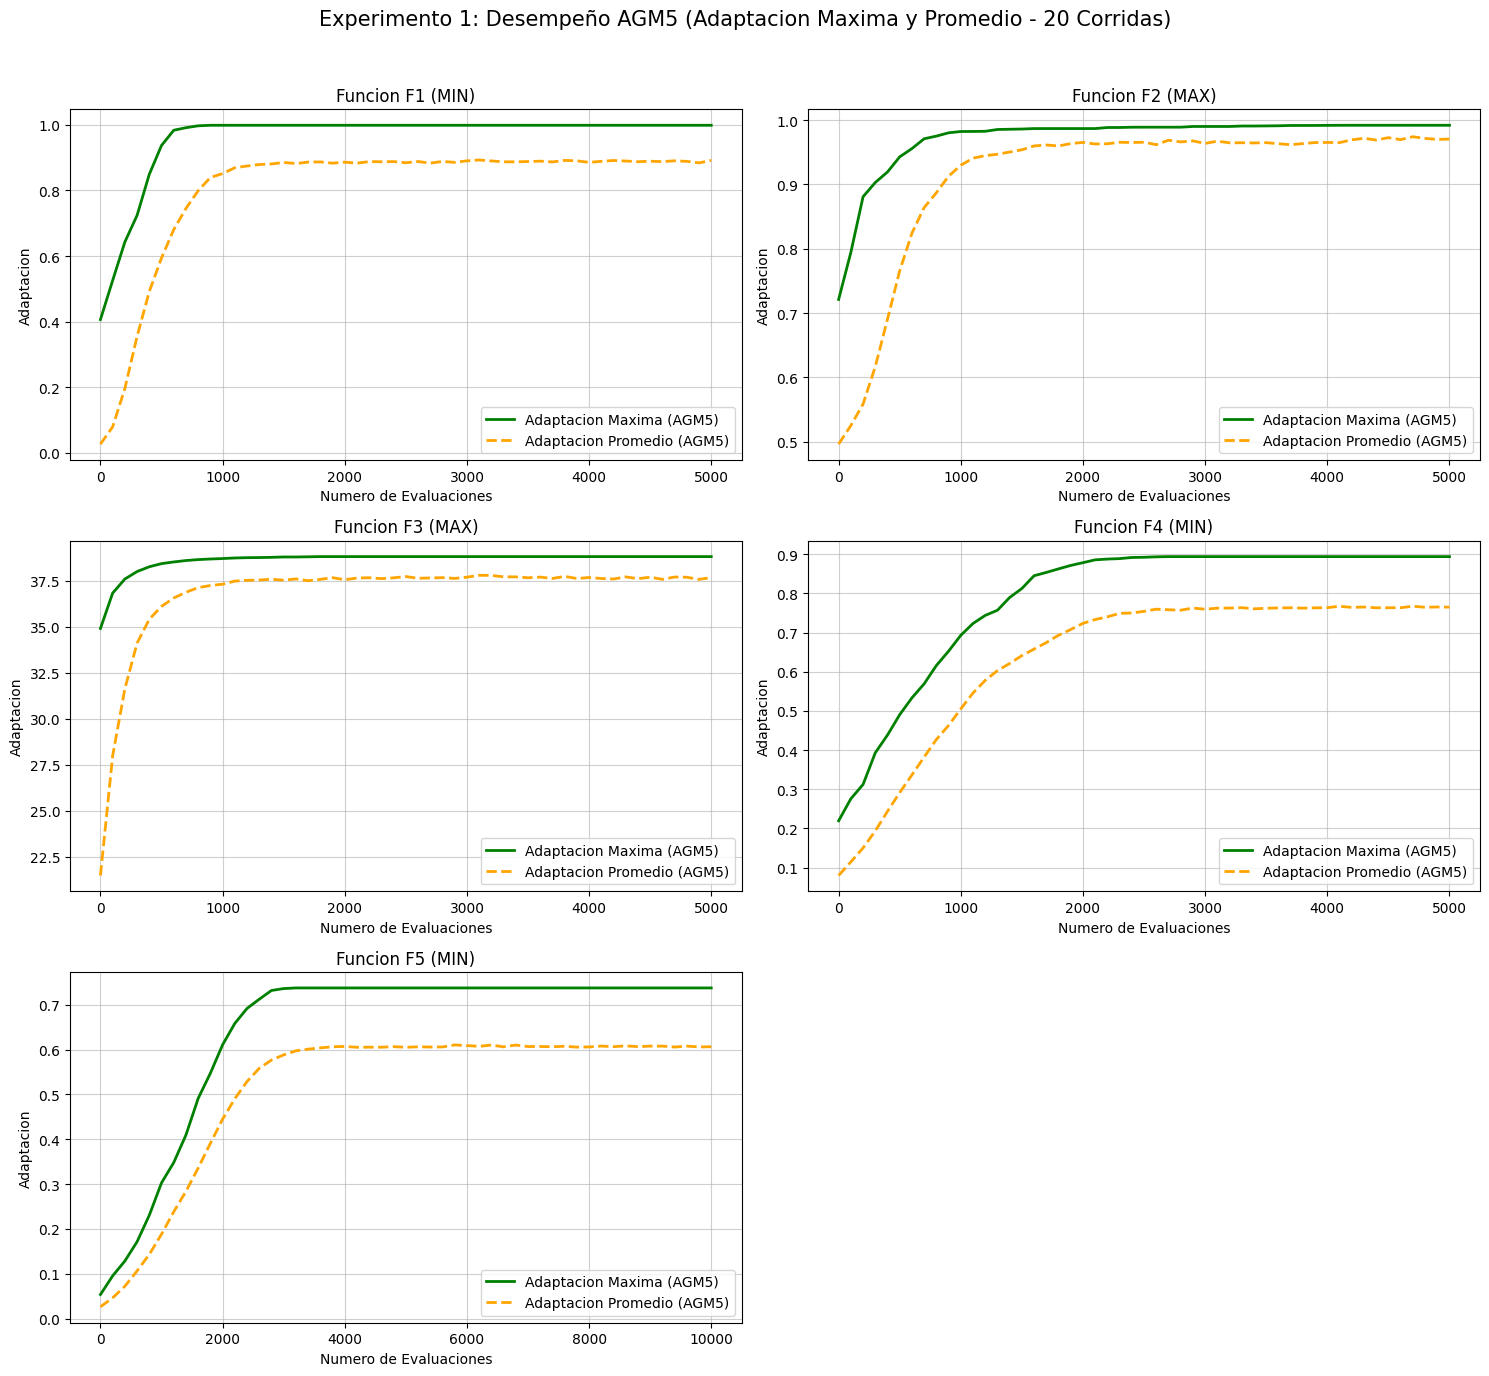
\includegraphics[width=0.95\textwidth]{resultados_1_1.png}%
    }{%
        \fbox{\parbox{0.9\textwidth}{\centering \vspace{1.2cm} \textit{[Colocar imagen como \texttt{output\_9\_1.png}: Desempeño AGM5 (Adaptación Máxima y Promedio - 20 Corridas)]} \vspace{1.2cm}}}%
    }
    \caption{Adaptación máxima y adaptación promedio del AGM5 en función del número de evaluaciones (promedio de 20 corridas).}
    \label{fig:exp1_agm5}
\end{figure}

\begin{figure}[H]
    \centering
    \IfFileExists{resultados_1_2.png}{%
        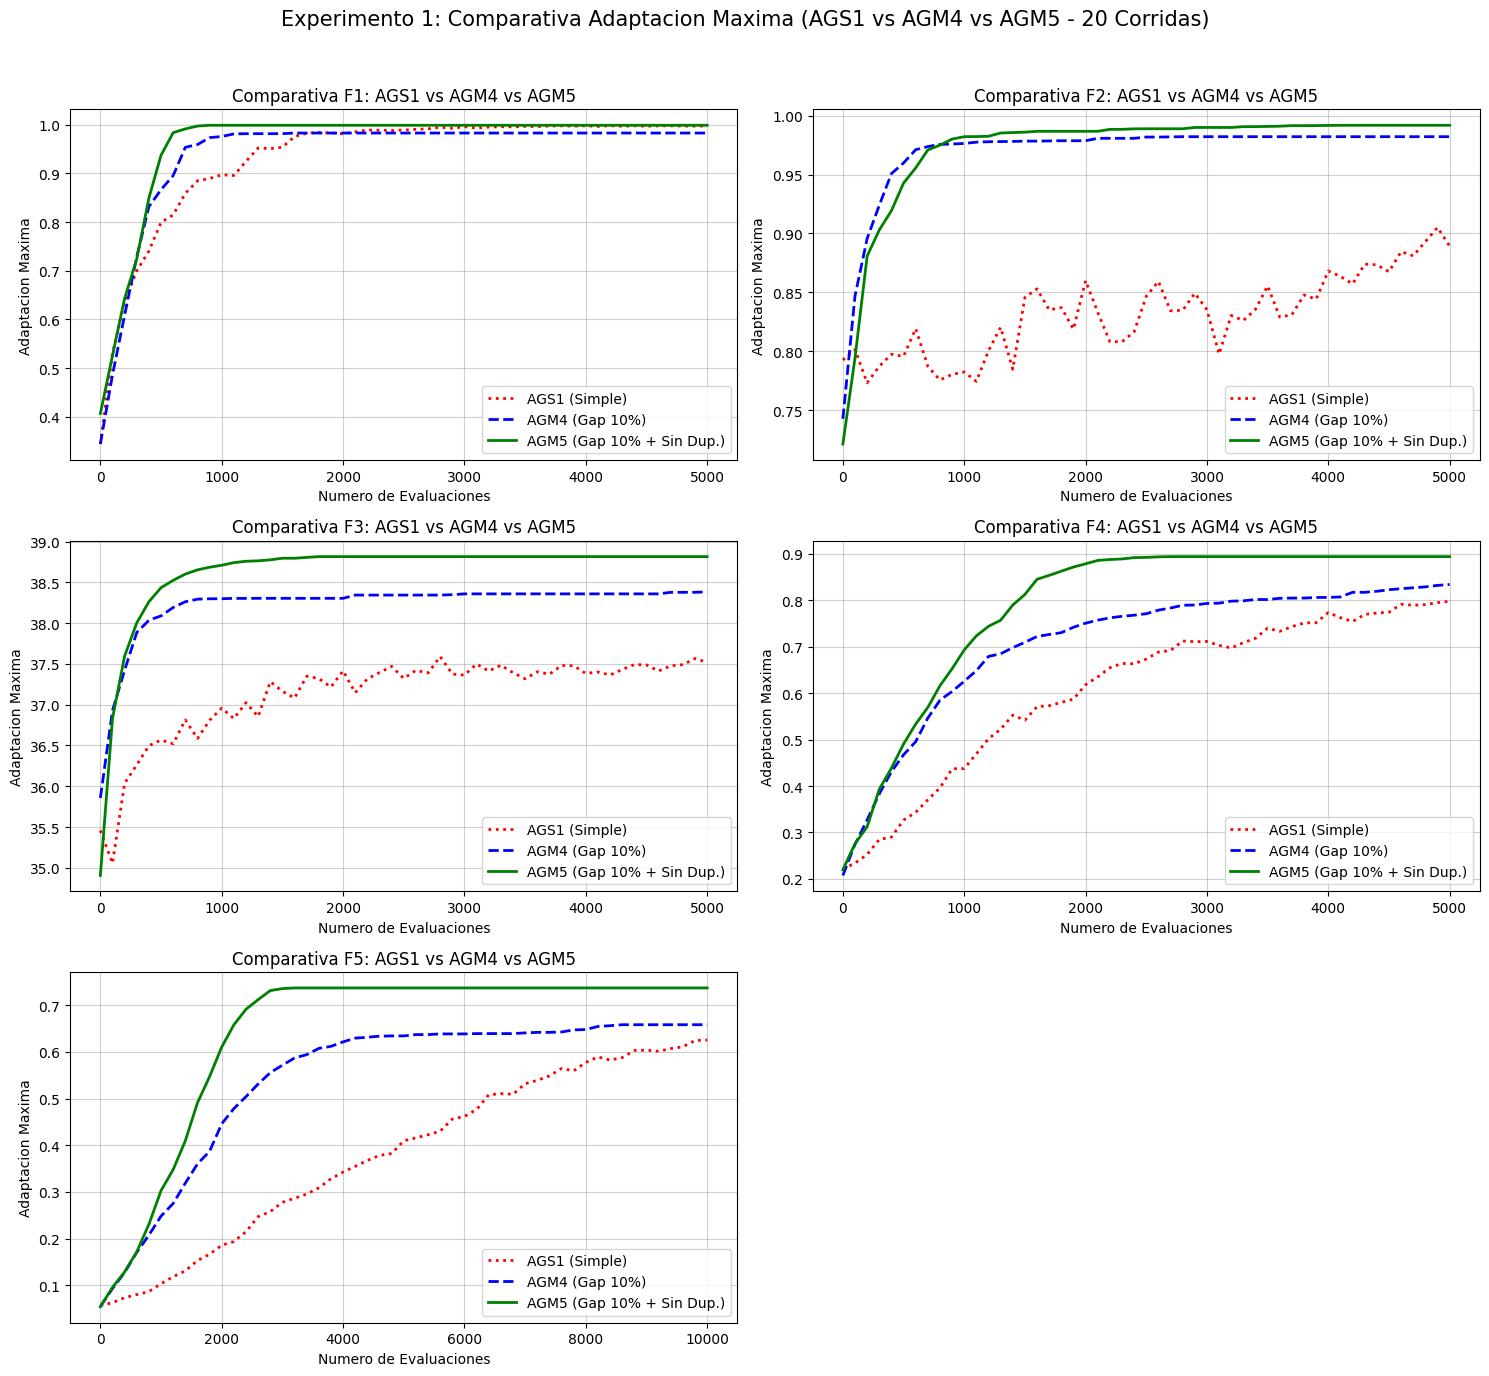
\includegraphics[width=0.95\textwidth]{resultados_1_2.png}%
    }{%
        \fbox{\parbox{0.9\textwidth}{\centering \vspace{1.2cm} \textit{[Colocar imagen como \texttt{output\_9\_2.png}: Comparativa Adaptación Máxima AGS1 vs AGM4 vs AGM5 - 20 Corridas]} \vspace{1.2cm}}}%
    }
    \caption{Comparación de la adaptación máxima entre AGS1, AGM4 y AGM5 en función del número de evaluaciones (promedio de 20 corridas).}
    \label{fig:exp1_comp}
\end{figure}

\subsection{Desempeño del algoritmo al introducir mejoras}

Para la segunda parte se seleccionó la función $F_2$ y se evaluaron los cinco algoritmos (AGS1, AGM2, AGM3, AGM4 y AGM5) durante $20$ corridas de $5000$ evaluaciones cada una. Siguiendo los valores sugeridos, para AGS1, AGM2 y AGM3 se utilizó $P_c = 0.80$ y $P_m = 0.002$, mientras que para AGM4 y AGM5 se utilizó $P_c = 0.90$ y $P_m = 0.01$, probando porcentajes de sustitución de $1\%$, $5\%$ y $10\%$. En la Tabla \ref{tab:comparacion_gaps} se muestran los resultados obtenidos al variar el porcentaje de sustitución.

\begin{table}[H]
\centering
\caption{Comparación del porcentaje de sustitución ($1\%, 5\%$ y $10\%$) para AGM4 y AGM5 en $F_2$.}
\label{tab:comparacion_gaps}
\begin{tabular}{@{}c c >{\centering\arraybackslash}p{3.4cm} >{\centering\arraybackslash}p{3.4cm} c@{}}
\toprule
\textbf{Algoritmo} & \textbf{Gap (\%)} & \textbf{Adapt. Máx. Promedio Final} & \textbf{Mejor Valor $F_2(x,y)$ Alcanzado} & \textbf{Coordenadas $[x, y]$} \\ \midrule
     & 1\%  & 0.980024 & 0.999981 & $[-0.00305, \; 0.00305]$ \\
AGM4 & 5\%  & 0.979984 & 0.999981 & $[0.00305, \; -0.00305]$ \\
     & 10\% & 0.976210 & 0.999981 & $[-0.00305, \; -0.00305]$ \\ \midrule
     & 1\%  & 0.988490 & 0.999981 & $[-0.00305, \; -0.00305]$ \\
AGM5 & 5\%  & 0.991022 & 0.999981 & $[-0.00305, \; -0.00305]$ \\
     & 10\% & 0.990481 & 0.999981 & $[-0.00305, \; -0.00305]$ \\ \bottomrule
\end{tabular}
\end{table}

Como se observa en la Tabla \ref{tab:comparacion_gaps}, para el AGM4 el mejor promedio final se obtuvo con un porcentaje de sustitución de $1\%$ ($0.980024$), mientras que para el AGM5 el mejor desempeño se alcanzó con un porcentaje de sustitución de $5\%$ ($0.991022$). Utilizando estos mejores porcentajes de sustitución, en la Tabla \ref{tab:resumen_5_algs} y en la Figura \ref{fig:exp2_5algs} se presenta la comparación general de los cinco algoritmos.

\begin{table}[H]
\centering
\caption{Resumen del desempeño de los cinco algoritmos en la función $F_2$ (promedio de 20 corridas).}
\label{tab:resumen_5_algs}
\begin{tabular}{@{}l >{\centering\arraybackslash}p{3.4cm} >{\centering\arraybackslash}p{3.0cm} c@{}}
\toprule
\textbf{Algoritmo} & \textbf{Adapt. Máx. Final (20 corr.)} & \textbf{Mejor $F_2(x,y)$ Global} & \textbf{Coordenadas $[x, y]$} \\ \midrule
1. AGS1 (Simple)             & 0.910259 & 0.990284 & $[0.97964, \; -2.98166]$ \\
2. AGM2 (+ Renormalización)  & 0.930712 & 0.999981 & $[-0.00305, \; 0.00305]$ \\
3. AGM3 (+ Elitismo)         & 0.981748 & 0.999981 & $[0.00305, \; -0.00305]$ \\
4. AGM4 (+ Gap 1\%)          & 0.980024 & 0.999981 & $[-0.00305, \; 0.00305]$ \\
5. AGM5 (+ Sin Dup, Gap 5\%) & 0.991022 & 0.999981 & $[-0.00305, \; -0.00305]$ \\ \bottomrule
\end{tabular}
\end{table}

\begin{figure}[H]
    \centering
    \IfFileExists{resultados_2_1.png}{%
        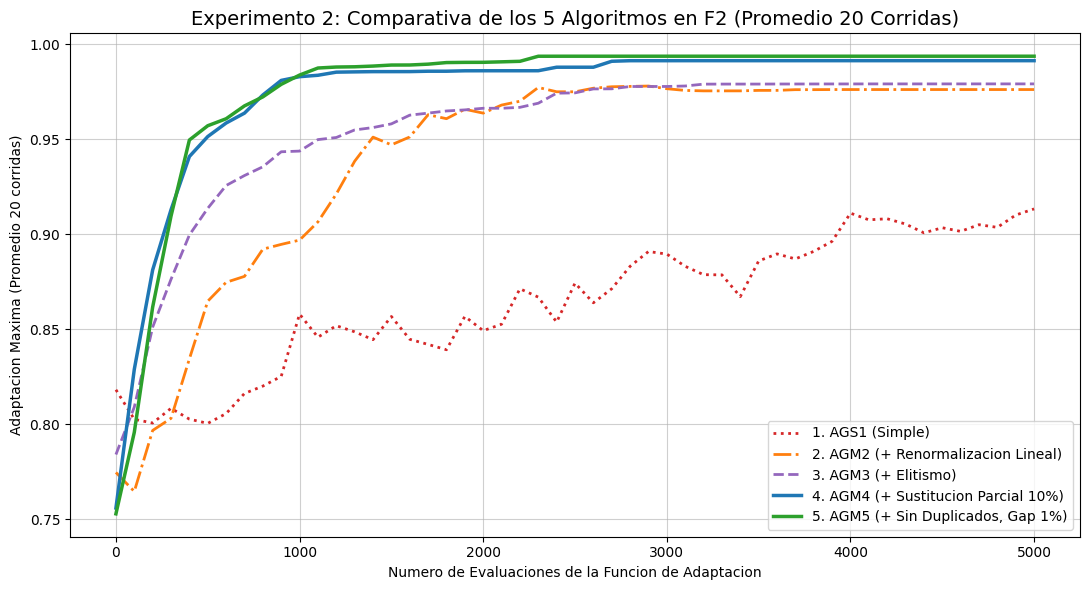
\includegraphics[width=0.90\textwidth]{resultados_2_1.png}%
    }{%
        \fbox{\parbox{0.9\textwidth}{\centering \vspace{1.2cm} \textit{[Colocar imagen como \texttt{output\_11\_1.png}: Comparativa de los 5 Algoritmos en F2 (Promedio 20 Corridas)]} \vspace{1.2cm}}}%
    }
    \caption{Comparación de la adaptación máxima en función de las evaluaciones de la función de adaptación para los cinco algoritmos en $F_2$.}
    \label{fig:exp2_5algs}
\end{figure}


\textbf{AGS1 a AGM2:} Con $P_c = 0.80$ y $P_m = 0.002$, el AGS1 tuvo un promedio bajo ($0.910259$) y no logró pasar de $0.990284$. Al agregar la renormalización lineal en el AGM2, se mantuvo una diferencia constante de selección entre los individuos ordenados y se logró alcanzar en al menos una corrida el óptimo de $0.999981$, subiendo la media a $0.930712$; sin embargo, al no tener elitismo, ambas curvas siguen presentando fuertes caídas entre generaciones.

\textbf{AGM2 a AGM3:} Al conservar al mejor individuo en el AGM3, desaparecen las caídas de la curva de adaptación máxima y el promedio de las $20$ corridas sube notablemente de $0.930712$ a $0.981748$.

\textbf{AGM4 y AGM5:} Como muestra la Figura \ref{fig:exp2_5algs}, tanto AGM4 como AGM5 crecen mucho más rápido en las primeras $500$ evaluaciones que el AGM3, debido a que los nuevos hijos entran de inmediato a la población sin esperar a que se evalúen $100$ individuos. No obstante, en el AGM4 la población tiende a llenarse de individuos repetidos y se estanca en un promedio de $0.980024$. Cuando se eliminan los duplicados en el AGM5 ($\text{Gap} = 5\%$), el algoritmo mantiene la diversidad de la población y consigue el mejor rendimiento global de todas las pruebas con un promedio de $0.991022$.



\end{document}